%%%
%%% Thesis
%%%
%%% Template Author:	Malte Hellmeier
%%% URL:						https://github.com/mhellmeier/LaTeX-Thesis-Template
%%%
% !TeX spellcheck = en_US 

% ****************************** %
% ********** Preambel ********** %
% ****************************** %
\documentclass[
	12pt,
	a4paper,
	american,
	oneside
	]{scrartcl}

% Add your packages in the packages.tex file
% ****************************** %
% ********** Packages ********** %
% ****************************** %

\usepackage[top=2.5cm, 
			bottom=2.5cm,
			left=2.5cm,
			right=2.5cm
			]{geometry}														% for page margins
\usepackage{lipsum}													  % lorem ipsum dummy text
\usepackage{pdflscape}												% for landscape pages (alternativ without PDF rotation: lscape)
\usepackage[onehalfspacing]{setspace} 					  % for line spacing
\usepackage[australian]{babel} 									 % set language
\usepackage[utf8]{inputenc}      								 % text is inserted in UTF-8
\usepackage[T1]{fontenc}         								   % use modern font encoding
\usepackage{lmodern}												 % use modern font
\usepackage{fancyhdr}												 % custom fancy header and footer
\usepackage{graphicx}            									  % useful graphic tool
\usepackage{tikz}														  % graphic tricks
\usepackage{array}               										 % for better tables
\usepackage{longtable}           									   % for tables, that span across multiple pages
\usepackage{nicefrac}            										% for nicer frations like 1/2
\usepackage{units}               										  % for nice printing of units like N or km/h
\usepackage{textcomp}            									  % for \textdegree to obtain °
\usepackage{enumitem}												  % enumeration in every level (legal)
\usepackage[autostyle,style=american]{csquotes}			% references, cites, ...
\usepackage{amsmath}												  % for mathamatic equations
\usepackage{xpatch}														% for customizations
\usepackage[
	backend=biber,
	natbib=true,
	style=authoryear,
	giveninits=true,
	eprint=false,
	doi=false,
	isbn=false,
	url=false,
	urldate=long,
	dateabbrev=false,
	date=year,
	labeldate=year,
	dashed=false,
	maxbibnames=99,
	maxcitenames=2,
	uniquelist=false
]{biblatex} % references
\addbibresource{literature.bib}
\usepackage{float}				 											% for floatings
\usepackage[printonlyused]{acronym} 						   % for acronyms
\usepackage{todonotes}			 									   % tool for todos | HINT: add [disable] option to disable without manual removal
\usepackage{multirow}			 										 % insert multi rows in tables
\usepackage{listings}			 										   % insert source code
\usepackage{color}				 											% insert source code
\usepackage{xcolor,colortbl}											% table cell coloring
\usepackage{tabularx}			 										  % for special tables
\usepackage{caption}													  % caption package
\usepackage{arydshln}			 										  % for dashed table lines
\usepackage[section]{placeins}	 									 % for placing floats in the correct section
\usepackage[pdfpagelabels=true,									   % for interactive PDFs; always load hyperref at the end
			hidelinks
			]{hyperref}

% Add your custom preamble code in the definitions.tex file
% ****************************** %
% ******** Definitions ********* %
% ****************************** %

% title & author
\title{\textbf{Thesis}}
\author{Your Name}


%\setlength{\parskip}{0.2cm} % space between paragraphs 
\setlength{\parindent}{0cm} % supress indent at the beginning of a new paragraph
\linespread{1.5} % add a 1.5 line spacing
\newcounter{pageCounter}

% start sections on a new page
\makeatletter
\renewcommand{\sectionlinesformat}[4]{%
	\ifstr{#1}{section}{\clearpage}{}%
	\@hangfrom{\hskip #2#3}{#4}%
}
\makeatother

% don't add appendix subsections to TOC
\appto\appendix{\addtocontents{toc}{\protect\setcounter{tocdepth}{1}}}
% reinstate the correct level for list of tables and figures
\appto\listoffigures{\addtocontents{lof}{\protect\setcounter{tocdepth}{1}}}
\appto\listoftables{\addtocontents{lot}{\protect\setcounter{tocdepth}{1}}}

% commands for links in the document
\newcommand\seclink[2]{\hyperref[#1]{#2}}
\newcommand\imglink[1]{\autoref{#1}}
\newcommand\tablelink[1]{\autoref{#1}}
\newcommand\urlfootnote[1]{\footnote{\url{#1}}}

% custom header and footer
\pagestyle{fancy}
\fancyhf{}
\fancyhead[L]{\slshape\nouppercase{\leftmark}}
\fancyfoot[R]{\thepage}

% prevent footnotes from splitting over several pages
\interfootnotelinepenalty=10000

% table definitions
% table caption
\makeatletter
\def\LT@makecaption#1#2#3{%
	\multicolumn{\LT@cols}{|c|}{\cellcolor{gray!40}\textbf{#2: }\textbf{#3}}%%%
}
\makeatother

% change treshhold for blockquotes
\SetBlockThreshold{1}

% allow lowercase acronyms in text but uppercase first letter in the list of abbreviations
% source: https://tex.stackexchange.com/a/70894/160825
\makeatletter
\newif\if@in@acrolist
\AtBeginEnvironment{acronym}{\@in@acrolisttrue}
\newrobustcmd{\LU}[2]{\if@in@acrolist#1\else#2\fi}
\newcommand{\ACF}[1]{{\@in@acrolisttrue\acf{#1}}}
\makeatother

% colouring source code
% source: https://stackoverflow.com/a/3175141/2056125
\definecolor{dkgreen}{rgb}{0,0.6,0}
\definecolor{gray}{rgb}{0.5,0.5,0.5}
\definecolor{mauve}{rgb}{0.58,0,0.82}

\lstset{frame=tb,
	language=Java,
	aboveskip=3mm,
	belowskip=3mm,
	showstringspaces=false,
	columns=flexible,
	basicstyle={\small\ttfamily},
	numbers=left,
	numberstyle=\tiny\color{gray},
	keywordstyle=\color{blue},
	commentstyle=\color{gray},
	stringstyle=\color{mauve},
	breaklines=true,
	breakatwhitespace=false,
	postbreak=\mbox{\textcolor{red}{$\hookrightarrow$}\space},
	tabsize=3,
	xleftmargin=5.0pt,
	xrightmargin=11.5pt
}

% define legal for enumeration in every level
\newlist{legal}{enumerate}{10}
\setlist[legal]{label*=\arabic*.}


% change URL visited text in the list of references
\DefineBibliographyStrings{english}{
	urlseen = {Accessed:} 
}
% try to create MISQ citation style
% source: https://github.com/pcbouman-eur/misq-latex-style
\renewcommand*{\nameyeardelim}{\addspace}
\let\oldcitet\citet
\renewcommand{\citet}[1]{\textsc{\oldcitet{#1}}} % make family name upper case in \citet

\renewcommand*{\newunitpunct}{\addcomma\space}

\DeclareNameAlias{sortname}{family-given}
\DeclareDelimFormat[bib,biblist]{nametitledelim}{\addperiod\space}

\renewcommand*{\intitlepunct}{\addspace}

\renewbibmacro*{volume+number+eid}{%
	\setunit{\addspace}%
	\printtext[parens]{%
		\printfield{volume}%
		\setunit*{\addcolon}%
		\printfield{number}}%
	\setunit{\addcomma\space}%
	\printfield{eid}}

\DeclareFieldFormat{doi}{%
	\mkbibparens{%
		doi\addcolon\space
		\ifhyperref
		{\href{https://doi.org/#1}{\nolinkurl{#1}}}
		{\nolinkurl{#1}}}}

\renewbibmacro*{doi+eprint+url}{%
	\setunit{\addspace}%
	\iftoggle{bbx:doi}
	{\printfield{doi}}
	{}%
	\newunit\newblock
	\iftoggle{bbx:eprint}
	{\usebibmacro{eprint}}
	{}%
	\newunit\newblock
	\iftoggle{bbx:url}
	{\usebibmacro{url+urldate}}
	{}}


% Research question command
\newcommand\researchquestion{How should a LaTeX template be designed to work for your thesis?}

% ******************************** %
% ********** Document ********** %
% ******************************** %
\begin{document}
	% Force LaTeX to never go over the right margin
	\sloppy
	
	% ***** Front Page *****
	\pagenumbering{Roman}
	\thispagestyle{empty}
\begin{titlepage}
	\begin{center}
		\begin{tikzpicture}[remember picture,overlay]
			\node[anchor=north west,yshift=-1.5cm,xshift=2.3cm] % change this position
				at (current page.north west)
				{
\includegraphics[width=1\textwidth]{images/logo.jpg}};
		\end{tikzpicture}

		
		\vspace{4.5cm}
		
		\textbf{Thesis}
		
		\vspace{1cm}
		
		\begin{spacing}{2}
			\textbf{\Large The Title of the Thesis should be added in the Code of the Front Page File}\\
		\end{spacing}
	
		
		\vspace{2.2cm}
		
		XX Weeks Thesis as Part of the\\
		Your Study (M.\,Sc.) Degree\\
		at the University of XXX
		
		
		\vspace{6cm}
		
		\begin{table}[H]
			\begin{tabular}{m{8cm}l}
				Submitted on: \today           		&                                       \\
				By: Your Name            		& Supervisor 1: Prof. Dr. XXX \\
				From: Place of Birth, Country         		& Supervisor 2: XXX, M.\,Sc.  \\
				Matriculation Number: 123\,456\,789 	&                                      
			\end{tabular}
		\end{table}
	\end{center}	
\end{titlepage}


	\cleardoublepage
	
	% ***** Table of Contents *****
	\setcounter{page}{2}
	\begin{spacing}{1}
		\tableofcontents
	\end{spacing}
	
	
	% ***** List of Abbreviations *****
	\clearpage
	\markboth{List of Abbreviations}{List of Abbreviations}
	\phantomsection
	\addcontentsline{toc}{section}{List of Abbreviations}
	\section*{List of Abbreviations}
	\begin{spacing}{1}
		% ****************************** %
% ********** Acronyms ********** %
% ****************************** %

\begin{acronym}[-------------]
	\acro{AI}{Artificial Intelligence}
	\acro{IS}{Information Systems}
	\acro{ML}{Machine Learning}
	\acro{RQ}{\LU{R}{r}esearch \LU{Q}{q}uestion}
\end{acronym}


	\end{spacing}
	
	
	% ***** List of Figures ***** 
	\begin{spacing}{1}
		\clearpage
		\renewcommand{\listfigurename}{List of Figures}
		\markboth{List of Figures}{List of Figures}
		\phantomsection
		\addcontentsline{toc}{section}{List of Figures}
		\listoffigures
	\end{spacing}
	
	
	% ***** List of Tables *****
	\begin{spacing}{1} 
		\clearpage
		\renewcommand{\listtablename}{List of Tables}
		\markboth{List of Tables}{List of Tables}
		\phantomsection
		\addcontentsline{toc}{section}{List of Tables}
		\listoftables
	\end{spacing}
	
	
	\clearpage
	\setcounter{pageCounter}{\value{page}}
	\pagenumbering{arabic}
	
	
	% ********************************
	% ********* Introduction *********
	% ********************************
	\FloatBarrier
	\section{Introduction}\label{sec:introduction}
	Hello everyone! This thesis template is made for a seminar, bachelor, or master thesis. I will try to give you some examples of how to make your customer things. You will find them in the \seclink{sec:anotherSection}{Example Section} (see section \ref{sec:anotherSection}). More information, credits, references, license etc. can be found in the GitHub Repository\urlfootnote{https://github.com/mhellmeier/LaTeX-Thesis-Template}.
	
	
	% ********************************
	% ****** Literature Review *******
	% ********************************
	\clearpage
	\FloatBarrier
	\section{Literature Review}\label{sec:literatureReview}
	
	You can add your custom \ac{RQ} and use it in your document with \texttt{\textbackslash researchquestion}: \emph{\researchquestion}
	
	
	% ********************************
	% ****** Example Section ********
	% ********************************
	\clearpage
	\FloatBarrier
	\section{Example Chapter / Section}\label{sec:anotherSection}
	
	\subsection{Content}
	Some information about the content. You can make your text \textbf{bold} or \emph{italic}. You are also able to make some inline math (like $f(x)=m*x+b$ or $\frac{1}{2}$) or coding fonts (\texttt{yourCustomMethod()}). If you want to add additional sources, you can try to cite them directly in the text, like the popular publication \citet{hawking.1973}, or at the end of your sentence \citep[p.~1]{hawking.1973}. You are also able to make a blockquote:
	\blockquote{\grqq The result of design-science research in \acs{IS} is, by definition, a purposeful IT artifact created to address an important organizational problem. It must be described effectively, enabling its implementation and application in an appropriate domain\grqq\ \citep[p.~82]{hevner.2004}.}
	
	Sometimes you want to put additional information in a footnote\footnote{Great! You found the footnote!} or just a clickable URL\urlfootnote{https://github.com/mhellmeier/LaTeX-Thesis-Template}. I also added a crossref command like \seclink{sec:introduction}{Introduction} (you can click on the word \grqq \seclink{sec:introduction}{Introduction}\grqq). This is also possible for figures and tables, like \imglink{fig:figure1} or \tablelink{tab:table2}.
	
	When working with acronyms, simply put them in the \texttt{acronyms.tex} file. Then you can use them, like \ac{AI} or \ac{ML}. They will be defined at their first usage. If you add \ac{AI} and \ac{ML} again, it will only show the short form. But you can force to use the long form of \acl{AI}, too.
	
	
	\subsection{Tables, Figures \& Source Code}
	
	In the following, an example table, image and source code is presented.
	\bigskip
	
	\begin{figure}[!htb]
		\centering
		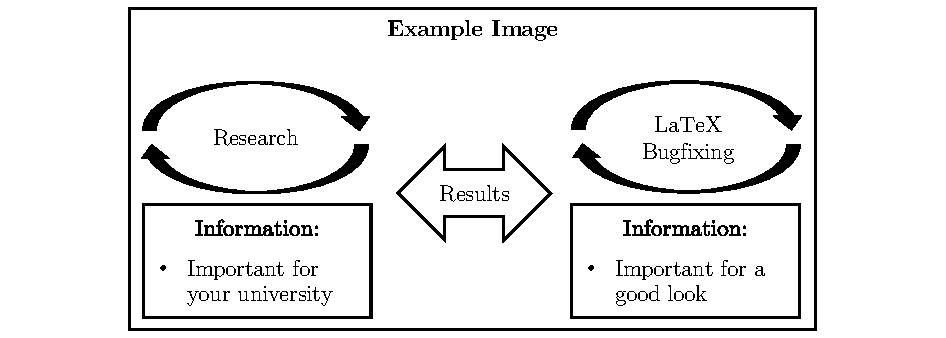
\includegraphics[width=1\textwidth]{images/example-image}
		\caption{Add a Caption for the Image}
		\label{fig:figure1}
	\end{figure}

	\begin{minipage}{\linewidth}
		\linespread{1}
		\begin{lstlisting}[caption={Hello World in Java},captionpos=b,label=source:helloWorld]
public class HelloWorld {
	
	public static void main (String[] args)	{
		// Old but Gold!
		System.out.println("Hello World!");
	}

}
		\end{lstlisting}
	\end{minipage}

	\small
	\begin{longtable}{|c|c|p{0.74\textwidth}|}
		\hline
		\caption{Add a Caption / Headline for your Table}\label{tab:table2}\\
		\hline
		\multicolumn{1}{|c|}{\cellcolor{gray!40}\textbf{No.}} & \multicolumn{1}{c|}{\cellcolor{gray!40}\textbf{Name}} & \multicolumn{1}{c|}{\cellcolor{gray!40}\textbf{Description}} \\ \hline
		\multicolumn{3}{|c|}{\cellcolor{gray!40}Multicolumn 1}\\  \hline
		1  & Category 1 & Add your description here \\ \hline
		2 & Category 2 & Lorem ipsum dolor sit amet, consetetur sadipscing elitr \\  \hline
		\multicolumn{3}{|c|}{\cellcolor{gray!40}Multicolumn 2} \\  \hline
		3 & Category 3 & Lorem ipsum dolor sit amet, consetetur sadipscing elitr \\  \hline
		4 & Category 4 & Lorem ipsum dolor sit amet, consetetur sadipscing elitr \\  \hline
	\end{longtable}

	\begin{landscape}
		\small
		\begin{longtable}{|c|c|p{20cm}|}
			\hline
			\caption{Landscape Table}\label{tab:table1}\\
			\hline
			\multicolumn{1}{|c|}{\cellcolor{gray!40}\textbf{No.}} & \multicolumn{1}{c|}{\cellcolor{gray!40}\textbf{Name}} & \multicolumn{1}{c|}{\cellcolor{gray!40}\textbf{Description}} \\
			1  & Category 1 & Add your description here \\ \hline
			2 & Category 2 & Lorem ipsum dolor sit amet, consetetur sadipscing elitr, sed diam nonumy eirmod tempor invidunt ut labore et dolore magna aliquyam erat, sed diam voluptua. \\  \hline
			\multicolumn{3}{|c|}{\cellcolor{gray!40}Multicolumn} \\  \hline
			3 & Category 3 & Lorem ipsum dolor sit amet, consetetur sadipscing elitr \\  \hline
			4 & Category 4 & Lorem ipsum dolor sit amet, consetetur sadipscing elitr, sed diam nonumy eirmod tempor invidunt ut labore et dolore magna aliquyam erat, sed diam voluptua. \\  \hline
			5 & Category 5 & Lorem ipsum dolor sit amet, consetetur sadipscing elitr, sed diam nonumy eirmod tempor invidunt ut labore et dolore magna aliquyam erat, sed diam voluptua. \\  \hline
		\end{longtable}
	\end{landscape}

	
	\subsection{This is a Subsection}
	
	\lipsum
	
	\subsubsection{This is a Subsubsection}
	
	\lipsum
	
	% ********************************
	% ********** Discussion **********
	% ********************************
	\clearpage
	\FloatBarrier
	\section{Discussion}\label{sec:discussion}
	
	\lipsum
	
	% ********************************
	% ********** Concluson **********
	% ********************************
	\clearpage
	\FloatBarrier
	\section{Conclusion}\label{sec:conclusion}
	
	\lipsum
	
	% ********************************
	% ********** References **********
	% ********************************
	\clearpage
	\FloatBarrier
	\markboth{References}{References}
	\phantomsection
	\addcontentsline{toc}{section}{References}
	
	% Removes parentheses around date / year
	% source: https://tex.stackexchange.com/a/40710/160825
	\xpatchbibmacro{date+extradate}{%
		\printtext[parens]%
	}{%
		\setunit{\addperiod\space}%
		\printtext%
	}{}{}
	
	\printbibliography
	
	
	% ********************************
	% *********** Appendix **********
	% ********************************
	\FloatBarrier
	\appendix
	\section{Appendix}
	\markboth{Appendix}{Appendix}
	
	Add your content.
	
	\subsection{Subsection in Appendix}
	
	Add your content.
	
	\subsubsection{Another Level}
	
	Add your content.
	
	
	
	% ********************************
	% ******** Certification **********
	% ********************************
	\section*{Certification}
	\markboth{Certification}{Certification}
	``Your individual certification (made this work on your own etc.).''
	\paragraph{}$~~$\\
	\paragraph{}$~~$\\
	%Your City, \today\\
	\noindent\rule{5cm}{.4pt}\hfill\rule{5cm}{.4pt}\par
	\noindent Place, Date \hfill Signature 

\end{document}